\documentclass[12pt,a4paper]{article}

% Useful packages for article:
\usepackage{amsmath, amssymb, amsfonts, amsthm}
\usepackage{graphicx}
\usepackage[round]{natbib}
\usepackage[usenames,dvipsnames]{xcolor}
\usepackage{bm}
\usepackage{subfigure}
\usepackage{graphicx}
\usepackage{mathabx}
\usepackage{multirow}
\usepackage{setspace}
\usepackage{tabls,calc}
\usepackage{float}
\usepackage{parskip}
\setcounter{tocdepth}{5}
\setcounter{secnumdepth}{5}
\numberwithin{equation}{section}
\numberwithin{figure}{section}
\numberwithin{table}{section}
\floatstyle{ruled}
\restylefloat{table}
\restylefloat{figure}

%Theorem, Lemma, etc. environments
\newtheorem{theorem}{Theorem}%[section]
\newtheorem{lemma}[theorem]{Lemma}
\newtheorem{proposition}[theorem]{Proposition}
\newtheorem{corollary}[theorem]{Corollary}
\newtheorem{result}[theorem]{Result}

\newcommand{\floatintro}[1]{

  \vspace*{0.1in}

  {\footnotesize

    #1

    }

  \vspace*{0.1in}
}
\usepackage[pdftex, pdfusetitle, plainpages=false, 
				letterpaper, bookmarks, bookmarksnumbered,
				colorlinks, linkcolor=Sepia, filecolor=Blue, urlcolor=Blue, citecolor=Violet]
				{hyperref}

\makeatletter

%%%%%%%%%%%%%%%%%%%%%%%%%%%%%%%%%%%%%%%%%%%%%%%%%%%%%%%%%%%%%%%%%%%%%%%
%
%  Floats
%
%%%%%%%%%%%%%%%%%%%%%%%%%%%%%%%%%%%%%%%%%%%%%%%%%%%%%%%%%%%%%%%%%%%%%%%%
%
%  \c@topnumber            : Number of floats allowed at the top of a column.
\setcounter{topnumber}{8}
%
%  \topfraction            : Fraction of column that can be devoted to floats.
\renewcommand\topfraction{1}
%
%  \c@bottomnumber, \bottomfraction : Same as above for bottom of page.
\setcounter{bottomnumber}{3}
\renewcommand\bottomfraction{.8}
%
%  \c@totalnumber          : Number of floats allowed in a single column,
%                          including in-text floats.
\setcounter{totalnumber}{8}
%
%  \textfraction         : Minimum fraction of column that must contain text.
\renewcommand\textfraction{0}
\renewcommand\floatpagefraction{.9}
%
%  \c@dbltopnumber, \dbltopfraction : Same as above, but for double-column
%                          floats.
\setcounter{dbltopnumber}{6}
\renewcommand\dbltopfraction{1}
\renewcommand\dblfloatpagefraction{.9}
%
\pretolerance=8000
\tolerance=9500
\hfuzz=0.5pt
\vfuzz=2pt
\hbadness=8000
\vbadness=8000
%\newcommand{\nohyphens}{\hyphenpenalty=10000\exhyphenpenalty=10000}
\def\endcolumn{\parfillskip=0pt\par\newpage
   \noindent\parfillskip=0pt plus 1fil{}}

\newsavebox\ruledbox
\newlength \ruledlength
\ruledlength\linewidth 
\newcounter{box}
\renewcommand \thebox{\@arabic\c@box}
\def\fps@box{tbp}
\def\ftype@box{1}
\def\ext@box{lob}
\def\boxname{Box}
\def\fnum@box{\boxname~\thebox}
\@ifundefined{color}{%
\newenvironment{thinbox}
 {\fboxsep6pt
  \setlength\ruledlength{\linewidth-2\fboxsep-2\fboxrule}
  \begin{lrbox}{\ruledbox}
   \begin{minipage}{\ruledlength}
   \def\@captype{box}}
 {\end{minipage}\end{lrbox}
  \@float{box}
   \fbox{\usebox{\ruledbox}}
  \end@float}
\def\endcolumn{\parfillskip=0pt\par\newpage
   \noindent\parfillskip=0pt plus 1fil{}}
% CVR's two-column box
\newenvironment{widebox}
 {\fboxsep6pt
  \setlength\ruledlength{\textwidth-2\fboxsep-2\fboxrule}
  \begin{lrbox}{\ruledbox}
   \begin{minipage}{\ruledlength}
   \def\@captype{box}}
 {\end{minipage}\end{lrbox}
  \@dblfloat{box}
   \fbox{\usebox{\ruledbox}}
  \end@dblfloat}
}{%
\definecolor{linecolor}{rgb}{0,0,.6}
\definecolor{bgcolor}{rgb}{1,.894,.769}
\newenvironment{thinbox}
 {\fboxsep6pt%\fboxrule2pt
  \setlength\ruledlength{\linewidth-2\fboxsep-2\fboxrule}
  \begin{lrbox}{\ruledbox}
   \begin{minipage}{\ruledlength}
   \def\@captype{box}}
 {\end{minipage}\end{lrbox}
  \@float{box}
   \fcolorbox{linecolor}{bgcolor}{\usebox{\ruledbox}}
  \end@float}
\def\endcolumn{\parfillskip=0pt\par\newpage
   \noindent\parfillskip=0pt plus 1fil{}}
% CVR's two-column box
\newenvironment{widebox}
 {\fboxsep6pt\fboxrule1pt
  \setlength\ruledlength{\textwidth-2\fboxsep-2\fboxrule}
  \begin{lrbox}{\ruledbox}
   \begin{minipage}{\ruledlength}
   \def\@captype{box}}
 {\end{minipage}\end{lrbox}
  \@dblfloat{box}
   \fcolorbox{linecolor}{bgcolor}{\usebox{\ruledbox}}
  \end@dblfloat}
}
\makeatother
  
\title{Deep Graph Kernels\thanks{Thesis proposal} }

\author{Pankaj Kumar\thanks{Skolkovo Institute of Science and Technology, Skolkovo Innovation Center, Building 3, Moscow  143026 Russia. Email: \url{pankaj.kumar@skolkovotech.ru}}} 


\date{}

\begin{document}
\maketitle
\begin{abstract}
We intend to build hybrid statistical agent based model, which can be interchangeably used as statistical or agent based model. The interchanging between models solves the problem of validation, calibration, parameter estimation and simulation complexity, as they are only used when required. The empirically grounded agent based model, cluster the agents based on trading strategies using dynamic machine-learning method called smooth plaid clustering technique. The novel method maps trading strategies of all traders in a highly liquid, anonymous electronic market to find certain common strategies belonging to common cluster. This in turn describes behaviour of agents who inhabit the new ecosystem of an anonymous electronic financial market. Then, we examine the price dynamics by knocking out agent one by one.
\end{abstract}
%\par
%\noindent
%\textbf{Keywords:} Agent Based Model $\cdot$ High Frequency Trading $\cdot$ Agent Ecology $\cdot$ Trading Strategies $\cdot$ CDA \\
%\\
%\textbf{JEL Classification:} G10 $\cdot$ C12
%\newpage
%\tableofcontents
%\newpage
\section{Introduction}
Financial markets are viewed as (macroscopic) complex systems with an internal (microscopic) structure consisting of many agents interacting so as to generate the systemic property. This complexity represents big challenges for researchers to decipher the market microstructure. The traditional mainstream analytical models from economics (econometric, DSGE etc.) posses serious difficulties in analysing market \citep{farmer2009}. By facilitating bottom-up approach, agent based models (ABM) models complex system by introducing behavioural rules, non-linear interactions, networks and bounded rationality. The current research in ABM have diverse range of intentions like reproducing stylized facts \citep{Stanley1999, BouchaudPotters2004}, behavioural origin \citep{AlfiPietroneroZaccaria2009I, AlfiPietroneroZaccaria2009II, CristelliPietroneroZaccaria2009, FengLiPodobnikPreisStanley2012} crisis or bubble predication \citep{bonnet2005, KirilenkoKyleSamadiTuzun2010, harras2011,farmer2011} and traders behavior \citep{LuxMarchesi1999, ContBouchaud2000, chiarella2002}. This list is, of course, far from exhaustive, but they represents specific modeling trend. For other models, please refer \citet{CristelliPietroneroZaccaria2011, chak2011, samanidou2007, lebaron2006}. 
 
However, agent based models also comes with some criticisms about problem of validation, calibration, parameters estimation and simulation complexity. Adding to it, the major drawbacks of agent-based models is the lack of an analytical form \citep{LeombruniRichiardi2005}, robustness of simulation runs yielding sufficiency theorem \citep{Grazzini2011} and efficient estimation of the "empirical relevant" parameters \citep{BianchiCirilloGallegatiVagliasindi2007, Grazzini2011} is still largely missing in the literature.

emeprical abm integration  

The possible solution to check disadvantages of agent based model is to use it only when it is required, have efficient calibration and validation of model. This actually laid the foundation for "hybrid statistical agent based model"\footnote{The model can be interchangeably used as statistical, agent based model or both}, key advance in the design of empirically grounded agent based models of financial markets. 
 

\subsection{Motivation}
The propulsion force of taking this topic as graduate thesis is curiosity generated by the May 6, 2010 Flash Crash\footnote{See Kirilenko, Kyle, Samadi, and Tuzun, "The Flash Crash: The Impact of High Frequency Trading on an Electronic Market", \citet{kirilenko2010}} and high frequency trading \footnote{ see, \citet{arndt2011}}(HFT, HFT also refers to high frequency traders). According to estimates from the Tabb Group \footnote{See Tabb reports "Next-Generation Algorithms: High Frequency for Long Only", December 2010, Morgan, Cheyenne, \url{http://www.tabbgroup.com/PublicationDetail.aspx?PublicationID=795}}, HFT accounted for around 56\% of US equity trading in 2010, up from 21\% in 2005. Being a fairly new phenomenon, academic research on this subject is still limited in numbers and to some extent inconclusive with respect to potential risks posed by HFT. 

The not easy task of about the hypothesis on agent behaviour, directed our research look at high frequency agent resolved data in order to build, validate, estimate and/or calibrate the ABM. 

\subsection{Objective}

Evolutionary progress requires the knowledge of the past to look for the future; it is necessary to use, when necessary, complex computational models without forgetting the lessons taught by analytical modelling. Keeping above statement in mind, this proposal seeks to extend traditional statistical model to empirical agent based modelling, to improve reliability of agent-based models and communication among different modelling methodologies. The approach focuses on expressiveness and descriptiveness, and thus has been strongly driven by data.Our thesis project has three main lines of research. 

The modelling of complex system (\citep{Arthur1994}), especially, financial market is largely influenced by agent based modelling. Despite many investigated agent based models (complete list, refer (\citep{ChakrabortiTokePatriarcaAbergel2011II}), only in few cases (\citep{TumminelloLilloPiiloMantegna2012}) an empirical investigation of agent strategies is done due to inaccessible data. Also, existing models take into account of agent's heterogeneity, analytical tractability or strategics, it need to be verified empirically to validate underlying assumption. The classification of agent validated through data mining exercise give strong foundation to empirically grounded agent based model. Our first objective is to do {\it agent cluster} using dynamic machine-learning method, named as "Smooth Plaid Clustering Technique" (\citep{ShawnMichailidiszKirilenko2011}). 

Based on empirically validated agent, our second research goal is to build {\it hybrid statically agent based model}, which can be used interchangeably, when required. The interchanging between statistical and ABM solves the problem of validation, calibration, parameter estimation and simulation complexity, as they are used only when required.

Third goal is to investigate the price dynamics by knocking out empirically verified agent one by one. Also, to examine the mechanical impact (\cite{FarmerZamani2007}) of cancelled, limit and partial order removal or addition. 

\section{Agent Ecology} \label{section:agent ecology}

A simplified conception of a financial market includes a set of agents, a trading mechanism, and securities. In ABM,  agents are computer programs that contain certain heuristics and computational learning algorithms, with the intention of capturing particular aspects of traders behavior. The classification of agent in theoretical and computational models are motivated by theoretical considerations, results of surveys and direct investigations of the trading profile of classes of investors \citep{TumminelloLilloPiiloMantegna2012}. According to the earlier literature, the stylized class is fundamentalists and chartists \citep{LuxMarchesi1999}, contrarian \citep{chan1988} , momentum \citep{chan1996}, informed and uninformed \citep{grossman1976}.

Although existing models take into account of agent's heterogeneity, analytical tractability or strategics, it need to be verified empirically to validate underlying assumption. The empirical investigations which was difficult to realized in past are possible because of the availability of confidential high frequency data and efficient data mining technique. The classification of agent validated through data mining exercise give strong foundation to empirically grounded agent based model.

\subsection{Literature Review}

While modeling ABM, It is the author's assertion that to accurately represent market mechanism and agent behavior. For years, this kind of model was difficult to see in academic literature. \citet{TumminelloLilloPiiloMantegna2012} investigated special database to identify clusters of traders by using Statistically Validated Networks (SVN). Due to availability of a customer specialization, market member data allow the researcher to decipher trading strategies, such as contrarian or momentum trading \citep{LilloMoroVaglicaMantegna2008}, order splitting \citep{VaglicaLilloMoroMantegna2008, MoroVicenteMoyanoGerigFarmerLilloMantegna2009, RenZhou2011} and liquidity provision \citep{TothEislerLilloKockelkorenBouchaudFarmer2012}. Using order-level NASDAQ data, \citet{hasbrouck2010} constructed a measure of low-latency activity, hence low latency traders by identifying strategic runs, which are linked submissions, cancellations, and executions that are likely to be parts of a dynamic strategy. 

\citet{paddrik2012} modeled a more realistic simulated market with the goal of representing agent classes. The aim of his study was to contribute to the growing literature on understanding the events of May 6, 2010 and other less significant flash crashes, which suggest that the traders clusters and the combination of trading styles are responsible for these events. Motivated by studies of \citet{kirilenko2010}, \citet{paddrik2012} divided their agents into six category namely fundamental buyers and sellers, market maker, opportunistic, HFT and small traders. The classification of traders are done on the basis of trade speed, number of trades, position and market volume. The outcome of this design was empirically grounded zero ABM for E-Mini S\&P 500 validated by stylized facts.

With access to quality HFT database, cluster identification literature is populated with innovative machine learning methods to infer the trading strategies and behaviour of traders from empirical data. Recent paper by \citet{KirilenkoYangPaddrikHaynesToddBelingScherer2011} used Markov Decision Process and Inverse Reinforcement
Learning (IRL) based approach to characterize traders cluster, trader behavior or infer trading strategies. There approach captures key empirical properties of order book dynamics and yet remains computationally tractable. \citet{ShawnMichailidiszKirilenko2011} proposed Smooth Plaid Model to identify cluster of traders and trading outcomes that persist through time. The agents are clustered in the category as defined by \citet{kirilenko2010} in their seminal paper about flash crash. 
\subsection{Model}

\section{Hybrid Statistical ABM}
\section{Price Dynamics}
\section{Conclusions}
High-frequency trading (HFT, HFT also refers to high frequency traders) has recently drawn massive public attention fuelled by the U.S. May 6, 2010 flash crash \footnote{See Kirilenko, Kyle, Samadi, and Tuzun, "The Flash Crash: The Impact of High Frequency Trading on an Electronic Market", \citet{kirilenko2010}} and the tremendous increases in trading volumes of HFT strategies. It is characterized by large numbers of small orders in compressed periods, with positions held for extremely short duration is estimated to have accounted for as much as 78\% of total trading volume in 2009. According to estimates from the Tabb Group \footnote{See Tabb reports "Next-Generation Algorithms: High Frequency for Long Only", December 2010, Morgan, Cheyenne, \url{http://www.tabbgroup.com/PublicationDetail.aspx?PublicationID=795}}, HFT accounted for around 56\% of US equity trading in 2010, up from 21\% in 2005. Being a fairly new phenomenon, academic research on this subject is still limited in numbers and to some extent inconclusive with respect to potential risks posed by HFT. Given the proprietary nature of high-frequency trading firms, there is relatively little known in the public domain about how they operate. At the same time, their importance in financial markets has grown very quickly in the past decade. As a result, the public understanding of financial markets has fallen somewhat behind the times. The purpose of this paper is to establish a frame of reference to begin improving our understanding of the new dynamics of financial markets, of which high-frequency trading is a central contributor.

In order to offer a clear foundation for further discussions, section \ref{sec:hft} defines academic and regulatory definition of HFT. We then starts building ABM by discussing important building blocks of ABM one by one. Section \ref{sec:abm} enlist the important ABM in literature pertaining to HFT. Section \ref{sec:ae} discusses about the agent ecology and section \ref{sec:ts} give a detail review of trading strategies employed by HFT with real example taken from various stock exchange. The continuous double auction, an important market mechanism is discussed in the section \ref{sec:cda}. All the above unit of ABM discussed above combined to give architecture, which includes survey of representative ABM are reviewed in section \ref{sec:arch}. Section \ref{sec:con} concludes.   

\section{High Frequency Trading}\label{sec:hft}
There is no consensus over universally accepted definition of HFT. Among its defining characteristics are the fact that investments are held for very short periods of time and typically (but not necessarily) positions are not carried overnight. \citet{kearns2010} define HFT as investment strategies, where traders hold positions between 10 milliseconds and 10 seconds and have no over-night positions. The rapid submission of cancellations and deletions is necessary to realize small profits per trade. According to \citet{cvitanic2010}, "HFT typically refers to trading activity that employs extremely fast automated programs for generating, routing, canceling, and executing orders in electronic markets. HF traders submit and cancel a massive number of orders and execute a large number of trades, trade in and out of positions very quickly, and finish each trading day without a significant open position, meaning that little or no risk is carried over night, with obvious savings". List of other definitions for HFT in academic literature is well documented in the study by \citet{arndt2011}. Though, there is no general agreement on a single definition of HFT, but extensive list pilling over time help us to extract the main characteristics of these definitions that are non-contradictive in academic literature.

A working group on behalf of the Commodity Futures Trading Commission (CFTC) proposed a definition of high frequency trading which is based on four key criteria and which is designed to avoid regulatory arbitrage. The emphasis is on clear recognised legal interpretation, mechanical description of high frequency trading that is deliberately neutral regarding types of trading strategies and how they interact with the market place. According to CFTC Technical Advisory Committee \footnote{see CFTC Technical Advisory Committee Sub-Committee on Automated and High Frequency Trading – Working Group 1, \url {http://www.cftc.gov/ucm/groups/public/@newsroom/documents/file/wg1presentation062012.pdf}}, HFT is form of automated trading that employs:

\begin{enumerate}

\item algorithms for decision-making, order initiation, generation, routing or execution
\item low latency technology that is designed to minimise response times, including proximity or co-location services
\item high speed connections to markets or order entry
\item recurring high message rates (orders, quotes or cancellations), using one or more forms of objective measurement, including cancel-to-fill ratios, participant-to-market message ratios, participant-to-market trade volume ratios

\end{enumerate}

The definition is inline with Securities and Exchange Commission, USA \citet{SEC2010}, Committee of European Securities Regulators, Europe \citet{CESR2010}, Markets in Financial Instruments Directive (MiFID), Europe \citet{mifid2010} and Australian Securities \& Investment Commission \citet{ASIC2010} to name a few influential regulatory bodies.

\section{Agent Based Model}\label{sec:abm}
The agent-based approach seeks to program the behavior of individual traders in dynamic markets with asymmetric information,learning, and uncertainty combination that poses many insurmountable technical challenges from a theoretical perspective. It offers many more parameters that can be altered to generate different scenarios. It also facilitates the study of emergent properties of trader's interactions and particular classes of traders in isolation \citep{farmer2009}. It can also be used to cluster various market participants to from agent ecology, assign behavioral preferences, allow interaction and simulate their micro and macro behavior over time. In fact, with the advent of the time, ABM has proven to be a fruitful tool for financial market research. Many field of application can be identified under stylized facts reproduction, bubbles or cashes predication or as as artificial laboratories for measuring various performance.

\subsection{Econophysics models}
Although research in ABM started from a diverse range of intentions (reproducing stylized facts, crises or bubble predication, traders behavior etc.), much of the physics-inspired literature aims at behavioral origin of stylized facts. In contract to economic agent based models, \citet{lebaron2006} provides a review of models built with agents who can exchange shares of stocks according to exogenously defined utility functions reflecting their
preferences and risk aversion. By incorporating realistic behavior, \citet{ContBouchaud2000} models herding behavior with noise traders. \citet{LuxMarchesi1999}, propose an agent-based model in which fundamentalists, chartists or noise traders interacts in settings, where there is no order book structure to keep track of orders. \citet{chiarella2002} goes further in modeling of trading mechanism by taking account of limit orders submissions, cancellation and execution. Other representative model includes Kim and Markowitz \citep{markowitz1989}; Levy, Levy and Solomon \citep{levy1994}; Solomon, Levy and Huang \citep{huang2001}; Solomon and Weisbuch \citep{solomon2002} etc. This list is, of course, far from exhaustive, but they represents specific modeling trend. For other models, please refer \citet{CristelliPietroneroZaccaria2011, chak2011, samanidou2007, lebaron2006}.
 
\subsection{Minority game models}
According to \citet{gou2005}, "The Minority Games (MG) comprises an odd number of agents choosing repeatedly between the options of buying and selling a quantity of a risky asset. The agents continually try to make the minority decision, i.e. buy assets when the majority of other agents are selling, and sell when the majority of other agents are buying". The extension of MG by allowing a variable number of active traders at each timestep are discussed in 
\citet{gou2005, challet2000, challet2001, wiesinger2013, chak2011}.

Agent-based mix-game model \citep{gou2005} was used to predict financial time series by introduction of simple generic algorithm into the prediction methodology. Its empirical example was done to forecast Shanghai Index. Going further by building a virtual stock market with a large number of artificial interacting boundedly rational agents, \citet{wiesinger2013} developed a method to reverse engineer real-world financial time series using MG and its key variants, called \$-game and related majority games. Their approach was validated by out-of-sample predictions of directional moves of the Nasdaq Composite Index. For understanding market's positive and/or negative trends, crashes and bubble effects, \citet{bonnet2005} used real market data coupled into a minority game with different payoff functions to study the dynamics and the location of financial bubbles. For other models based on the concept of MG or extended MG, please refer to \citet{chak2011}.

\subsection{Model driven}

Based on model driven approach in ABM, \citet{cvitanic2010} construct an artificial stock market, in which low frequency traders are represented by human being and high-frequency traders by machines. Here, HF traders are interpreted as liquidity provider only. Their study justifies positive linkage between market quality and HFT trading. Extending seminal work of \citet{grossman1988} with HF-traders as intermediaries between aggressive traders and market makers, \citet{cartea2011} and \citet{jarrow2012} found that HFT reduces the revenues of aggressive traders by deteriorating transactions prices. Further, HFT increase price volatility. 

\subsection{Evolutionary models}

The Santa Fe Artificial Stock Market \citep{PalmerArthurHollandLeBaronTayler1994}, is one of the best-known
examples of evolutionary agent-based financial markets. The agents make trading decisions based on binary market descriptors, and their strategies evolve in order to maximize profitability. It also deal with the rate of evolution
of the strategies, and how this gives rise to different regimes; the rational expectations regime and a more complex regime, where bubbles and crashes may appear. For other evolutionary models please refer to studies by \citet{chen2001} and \citet{Pereira2009}.

\citet{harras2011} used simple ABM to investigate the emergence of bubble and the consequential crash in financial markets. The bounded rational agents continuously adapting their trading strategies to market regime use feedback mechanisms. This lead to the development of transient collective herding regimes resulting in unsustainable high prices that are then corrected by a crash. The feedback mechanism is as a result of two dominating learning mechanisms, namely adaptation and imitation; which by reinforcing each other, result in bubbles and crashes. The same can be applied in HFT too. 


\subsection{Empirically grounded}

\citet{mike2008} was first to propose advanced calibration on the market data as for order
placement and cancellation methods, thus laying the foundation for the most complete empirical model ABM. Though the model can be viewed as a very simple ABM in which all components of the model are validated against real data from e London Stock Exchange. It simulate price formation under a continuous double auction, and the statistical properties of the resulting simulated sequence of prices are compared to those of real data \citep{mike2008}.

\citet{paddrik2012}, create a zero-intelligence agent based model of e-Mini S\&P 500 futures market and validate the simulated market against empirically observed characteristics of price returns and volatility. They illustrate
the applicability of the simulation and present experimental results which examine the hypothesis for the cause of the May 6th 2010 Flash Crash.

Using real order book data from the Chi-X exchange, along with a number of agents to interact with that data, \citet{panayi2012} investigate the impact of using both simple, limited intelligence traders, along with a more realistic set of traders. Their paper introduces the concept of semi-synthetic modeling, which combines past data and agents in a single simulation, and intuitively should be closer to the real market than a pure agent-based model. It also focuses on short-term behavior of stock prices and study the returns at the transaction level.

\citet{farmer2011} study the impact of HFT on stability of the markets by employing an ecological microstructure perspective of financial markets. They argue that due the significant homogeneity and interdependence in HFT, only a few algorithms and their interactions may dominate the market dynamics and can lead to systemic risk. They further extend their argument to the underline cause of 1987 crash, the 2007 quant crisis and the 2010 flash crash.

Extending the behavior ABM to to a stochastic model, \citet{FengLiPodobnikPreisStanley2012} reproduce stylized facts. Their approach provides a possible behavioral explanation for stochastic models for financial systems
in general and provides a method to parameterize such models from market data rather than from statistical fitting.


\section{Agent Ecology}\label{sec:ae}


\section{Trading Strategies}\label{sec:ts}

The literature and empirical evidence concerning particular trading strategies employed by HFT is scarce. Market quality improving strategies(e.g. "market making" improves liquidity and "statistical arbitrage" improves price efficiency) are openly questioned by opponents of HFT \citep{arnuk2009}. 

There are number of different types of HFT strategies, but according to ASIC Concept Release \citep{ASIC2010} it is classified into following types of strategies (see figure \ref{fig:HFTS}).
\begin{figure}[ht]
\begin{center}
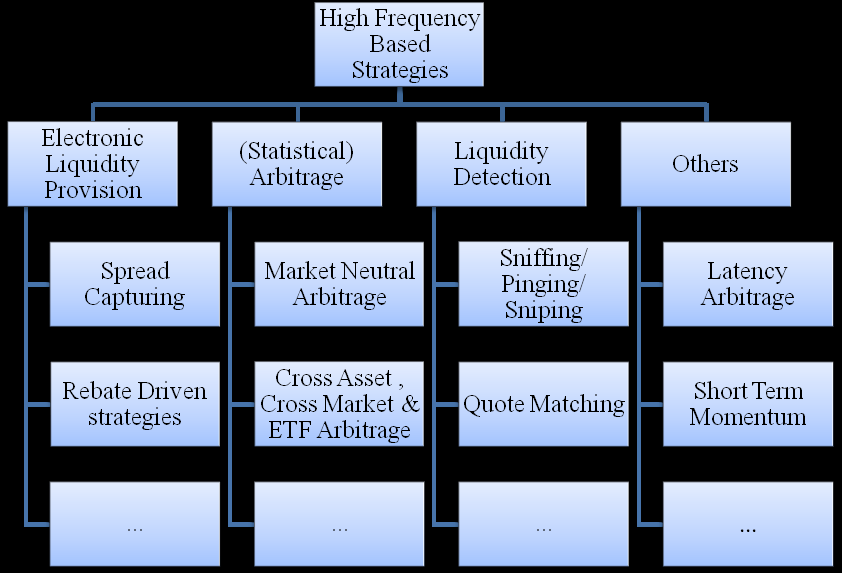
\includegraphics[width=\textwidth]{HFTS}
\caption{High Frequency Trading Strategies \citep{gomer2011}}
\label{fig:HFTS}
\end{center}
\end{figure} 

\subsection{Electronic Liquidity Provision}
It is most common strategies, where HFT act as liquidity providers. HFT liquidity providers have two basic sources of revenues: (i) They provide markets with liquidity and earn the spread between bid and ask limits and (ii) trading venues incentivize these liquidity provides by granting rebates or reduced transaction fees in order to increase
market quality and attractiveness \citep{gomer2011}. This strategies can be further classified into market making and rebate driven. 
\subsubsection{Market Making}
This strategy closely resembles its traditional counterpart of spread capturing. The liquidity providers profit from the spread between bid and ask prices by continuously buying and selling securities \citep{gomer2011}. So,intuitively, market makers reap profits by posting same size ask and bid order simultaneously, selling highly and buying low. Penn-Lehman-Automated-Trading (PLAT) simulator, which devised a market making strategy exploit market volatility without predicting the exact stock price movement direction \citep{lu2012}.

One improved variation of basic market making is smoked strategies \citep{lu2012}. In this, HFT place small misleading quotes to attract other side's market order. Once another party detects this quote, they will then send out a market order, which are only executed at the best market price, HFT can cancel the quotes before the 
market orders arrive, thus letting the other party hits the large shares previous posted by 
HFT. Figure \ref{fig:SS} illustrate one example of the smoking strategy. The author examined its existence by using the 5 days Hong Kong traded stock data. He found out that there are 20 occurrences happened in 5 days (7 bid side, 13 ask side). The average misleading quote size was 7,280 shares, the average cancellation duration was 1.98s, and the average trading volume was 2,160 shares. 

\begin{figure}[ht]
\begin{center}
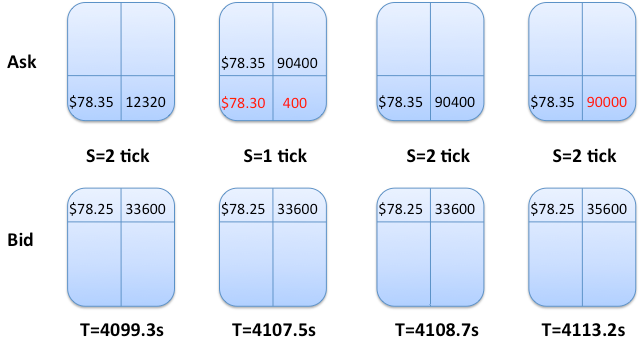
\includegraphics[width=\textwidth]{SS}
\caption{Example: Smoking Strategy \citep{lu2012}}
\label{fig:SS}
\end{center}
\end{figure}

\subsubsection{Rebate Trading} 
To attract liquidity traders, almost all market have adopted asymmetric pricing: members removing
liquidity from the market (taker; aggressive trading) are charged a higher fee while traders
who submit liquidity to the market (maker; passive trading) are charged a lower fee or are
even provided a rebate \citep{gomer2011}. The associated rebate for visible execution of 0.2 basis points (bps), \citet{gomer2011} estimated that the total rebate paid to makers on Chi-X in 2009 to amount to €17.4 million.

\subsection{ Statistical Arbitrage}
This strategy finds imbalances in prices on for example an correlated asset on single or different markets and profits on the difference. Historical data is analyzed for individual stocks and groups of assets in a search for trading patterns (within assets or across assets) that can be exploited for profit. These might represent temporary deviations from perceived patterns (e.g. pairs trading) or stem from identification of certain trading need in the market (e.g. a large trader that attempts to execute an order and temporarily changes the time-series behavior of prices).
\subsection{Liquidity Detection}
These trading strategies try to discern the patterns other market participants leave in the markets and feed on this kind of orders. Liquidity detectors algorithms primarily focus on large orders to detect sliced orders, hidden orders, orders being submitted by execution algorithms or to gain further information about electronic limit order books. Some of the popular algorithms are sniffing, pinging or sniping etc \citep{gomer2011}.

\subsection{Market Manipulative}
While the above legal trading strategies are used by various firms, there are still firms that conduct high frequency trading with strategies that are illegal. Oftentimes these HFT are the ones that get the most spotlight in the media and perhaps these strategies have cast an unfair cloud of distrust over HFT. We enlist some of them.

\subsubsection{Quote Stuffing}
According to \citet{NANEX2010}, "quote stuffing" is trading strategies involving immediate placement and cancellation of large number of orders. These intense episodic spikes in order submissions and cancellations was believed to be one important factors for flash crash \footnote{SEC Probes Canceled Trades, WSJ, July, 2010, \url{http://online.wsj.com/article/SB10001424052748703882304575465990082237642.html}}. In figure \ref{fig:QS}, starting from 9:30 a.m. until just after 9:51, there were, on average, 38 orders every second to buy or sell shares of Abbott Labs through the New York Stock Exchange. Then, in the span of one second, 10,704 orders hit Abbott and in the next second, another 5,483. And all but 14 of those combined orders were canceled within one second. \citet{egginton2011} examines the impact that intense episodic spikes in quoting activity on the market activity. There investigation revels that intense quote stuffing decreased liquidity, higher trading costs, and increased short term volatility. The above results was also justified by \citet{hasbrouck2012}. Market commentary by \citet{AES2012I} and \citet{AES2012II} give numerous examples to show quote stuffing with fairly different patterns. The common denominator is the massive number of new orders and cancellations hitting the market in a very short period of time. They use signal processing techniques to catch quote stuffing and other HFT scenarios. They also find that average spreads and volatilities are higher in the immediate aftermath of these events.
\begin{figure}[ht]
\begin{center}
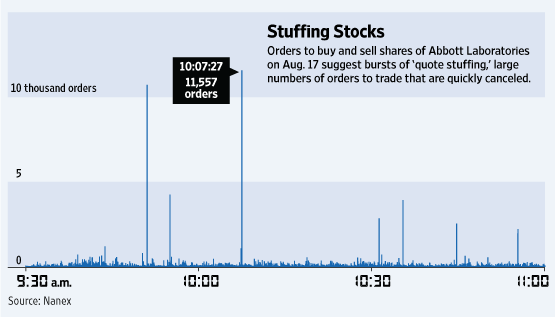
\includegraphics[width=\textwidth]{QS}
\caption{Quote Stuffing Example : Abbott Labs, 17th August, 2010 \citep{NANEX2010}}
\label{fig:QS}
\end{center}
\end{figure}

\subsubsection{Layering}
In the Future of Computer Trading in Financial Markets - Foresight, \citet{brogaard2011} define layering as an illegitimate strategy where, a trader places a number of sell orders at several price points and gives the false impression of strong selling pressure and drive the price down. Then, the trader buys at the cheaper price and cancels the sell orders. Thus by driving the price down, the trader can then buy the stock at an artificially cheap price and trade out when the book reverts.

Taking an example from \citet{brogaard2011} study to understand concept better, lets suppose a trader wants to buy a stock at 10.01, but its current bid is 10.02 and its ask is 10.03, it may put in a limit order to buy (a bid) at 10.01 that is hidden (or displayed). It will then place several limit orders to sell (offers) at a slightly higher price, say 10.05. Others will see that  there is strong selling pressure and will subsequently adjust their bids and offers lower. Once the  offer price hits 10.01 there will be a trade. The trader will have bought the stock for 10.01 and will withdraw his offer quotes.

\subsubsection{Order Book Fade}
Order book fade can be of two types "price" fade and "venue" fade. According to study by \citet{AES2012II}, "Price fade" refers to volume disappearing on a venue as soon as you trade there – e.g. after you buy the 100s, the 101s cancel immediately. The traders cancel orders in response to trades to avoid adverse selection. Figure \ref{fig:PF} shows a real example where a trade of 100@29.13 in Legrand SA on Euronext Paris lead to the 1200 shares at 29.135 being cancelled within milliseconds. Further, they find out that price fading is less frequent in case of wider spread. 
\begin{figure}[ht]
\begin{center}
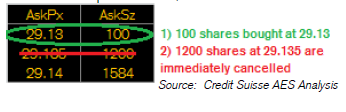
\includegraphics[width=\textwidth]{PF}
\caption{Price Fade Example : Legrand SA (Paris), September 21st, 2012 \citep{AES2012II}}
\label{fig:PF}
\end{center}
\end{figure}

Other form, “Venue fade” refers to volume disappearing immediately after a trade, but on a different venue from the executing venue. Similar to Price Fade, this may occur as traders cancel orders in response to trades across venues in order to avoid adverse selection. The example for the same is discussed in \citet{AES2012II}.

\subsubsection{Momentum ignition}
Momentum ignition refers to a strategy that attempts to trigger a number of other participants to trade quickly and cause a rapid price move. Generally, the instigator takes a pre-position; instigates other market participants to trade aggressively in response, causing a price move; then trades out \citep{AES2012II}. Momentum ignition is identified in the simple real world example (see \ref{fig:MI} ) using targeting volume spikes and outsized price moves. 

\begin{figure}[ht]
\begin{center}
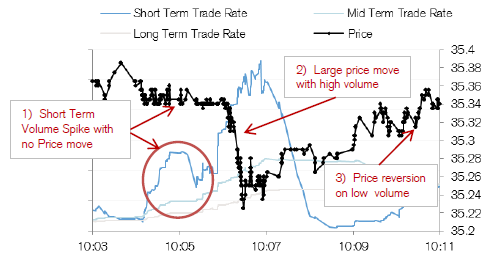
\includegraphics[width=\textwidth]{MI}
\caption{Momentum Ignition Identification : Daimler AG, 13th July, 2012 \citep{AES2012II}}
\label{fig:MI}
\end{center}
\end{figure}

\section{Continuous Double Auction}\label{sec:cda}
The continuous double auction (CDA) is an extensively studied topics in financial literature, for two main reasons. First, many actual stock, such as stock exchange (NYSE, LSE, NSE, NASDAQ etc), are of this type. Second, it provides a simple but effective model of a decentralized market for a asset. In CDA, buyers and sellers send their orders (price \& volume) at random times, which are collected in the order book. Depending on market regulations, traders may submit various kinds of orders, which includes limit orders( buy a specified quantity of a security at or below a given price, or to sell it at or above a given limit price)and market orders (buy or sell a specified quantity of a security at the best available price). The matching of the best bid (buy order) and the best ask (sell order) makes the trade happens. CDA mechanism is illustrated in the figure \ref{fig:CDA}
\begin{figure}[ht]
\begin{center}
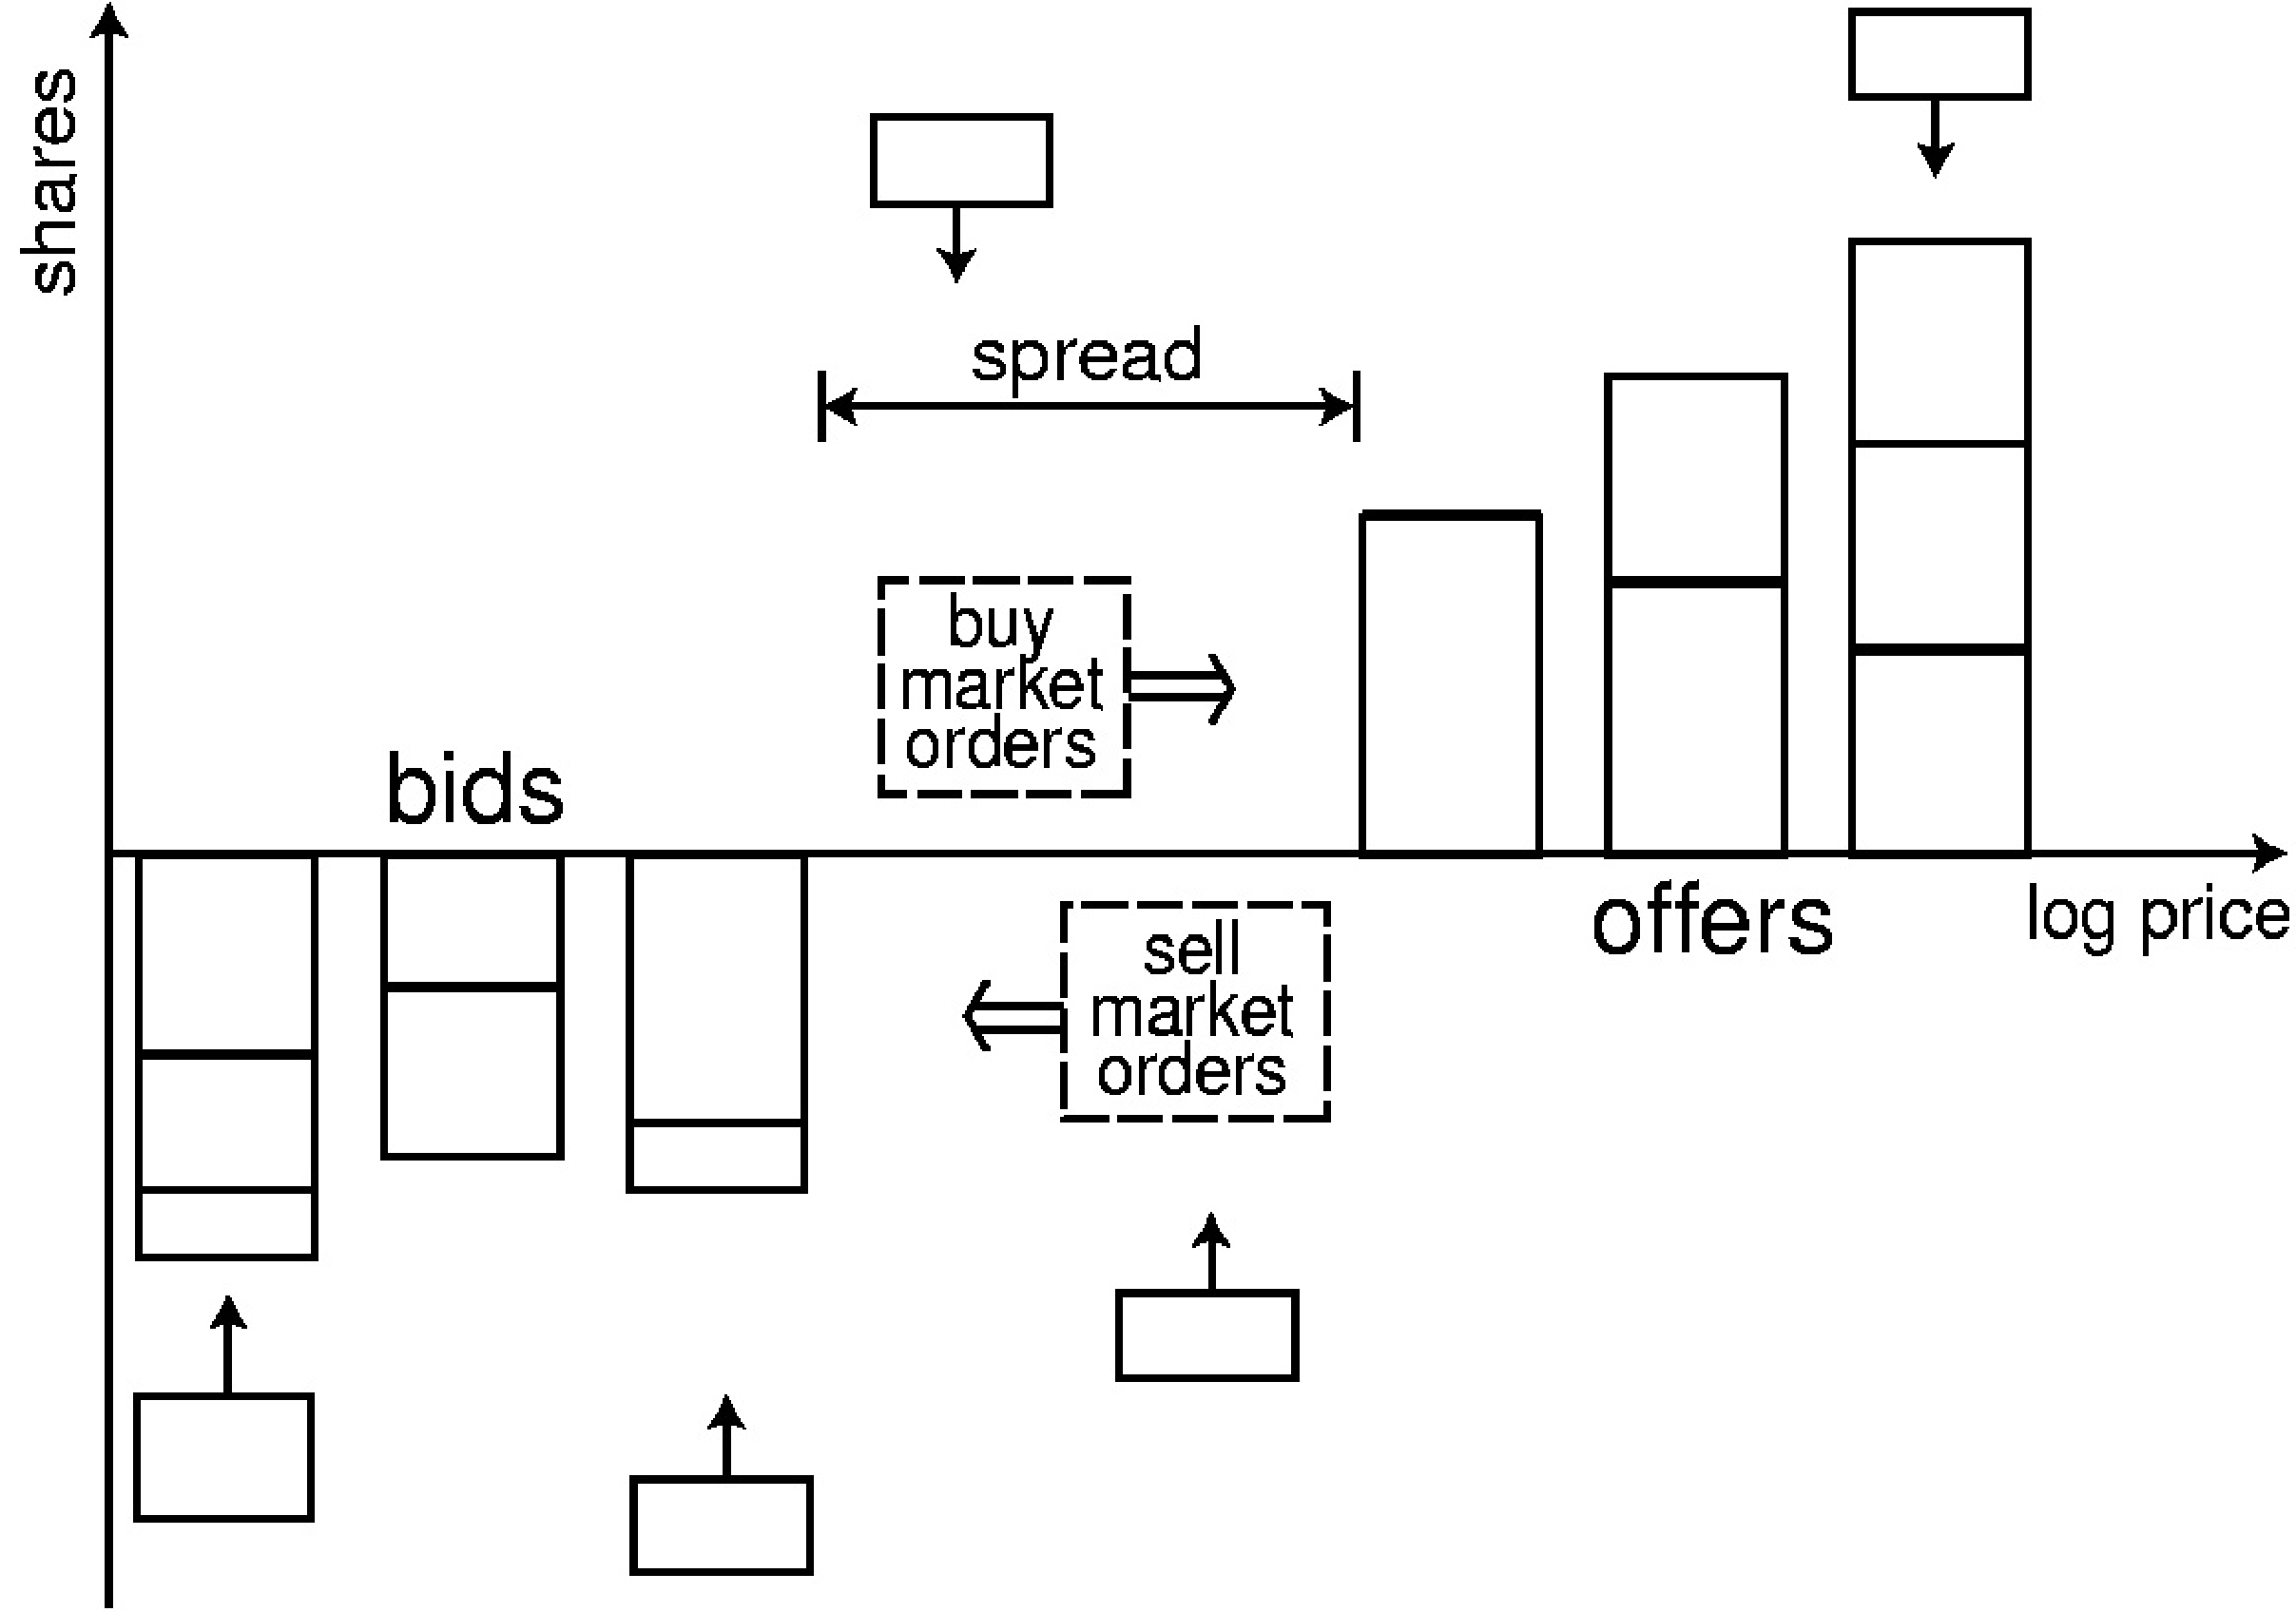
\includegraphics[width=\textwidth]{CDA}
\caption{A schematic illustration of the continuous double auction mechanism reproduced from \citet{SmithFarmerGillemotKrishnamurty2003}.}
\label{fig:CDA}
\end{center}
\end{figure}

The ever increasing number of CDA models with huge variations among them make it a daunting task for researcher who wishes to survey the entire literature. We survey some representative models for continuous double-auction markets through computational agents. The models are enlisted under methodology used. 

\subsection{Heterogeneous Agents}
\citet{chiarella2002} introduced an CDA mechanism with heterogeneous agents. They set bids and asks and post market and limit orders according to certain pre-defined rules. In Chiarella and Iori model, agent trade single asset. The orders arrive at the market sequentially, rather Poisson arrival. The demands of agents consist of three components, a fundamentalist component, a chartist component and a noise-induced component. Market dynamics of the model is well explained in \citet{chiarella2002}. Through numerical simulations, authors investigates, how price dynamics and spread are affected by liquidity, tick size and the average life of an order.

\subsection{Statistical Model}
Strictly speaking,  CDA model by \citet{SmithFarmerGillemotKrishnamurty2003} is more of a statistical random model than an agent-based one. The most amazing feature of the their model is that, although it is very simple (completely random and zero-intelligence), it has the power to simulate the evolution of the seemingly complex structure of CDA markets \citep{guo2005}.

\subsection{Evolutionary Game Theory}
\citet{Vytelingum2006}, investigate the effectiveness of different types of bidding behaviour (neutral, passive and aggressive) for trading agents in the Continuous Double Auction (CDA)using an evolutionary game-theoretic
analysis to determine the population dynamics of agents. Walsh \citep{Vytelingum2006} also use an evolutionary game-theoretic analysis in CDA mechanism to examine the interaction of a number of common strategies. It provides 
an insight on the population proportion that will adopt each strategy.
\subsection{Queuing Theory}
\citet{cont2010} introduced a stochastic model for the continuous-time dynamics of a limit order book based on the queuing theory. The purpose of the paper was to captures key empirical properties of order book dynamics and
its analytical tractability allows for fast computation of various quantities of interest without resorting to
simulation. The model on validation with high frequency data from Tokyo stock exchange, captures accurately the short term dynamics of the limit order book. They went further to model CDA using a Markovian queueing system \citep{cont2011}. The analytical results from the study provides some insight into the relation between order 
flow and price dynamics. These models can be used to asses the relevance of statistical equilibrium in stock market to investigate effect of market microstructure on book and price dynamics. 

\subsection{Real Models Implementation}
All the above models provide interesting insights into the price formation process but contain unobservable
parameters that govern agent preferences. Thus, they are difficult to estimate and use in applications \citep{cont2010}. Empirical studies by \citet{TothEislerLilloKockelkorenBouchaudFarmer2012, FarmerZamani2007, Bouchaud2002, Farmer2004} provides  extensive list of statistical  features of CDA, which are challenging to incorporate in a single model, but still need to be included.
 
For example, \citet{scalas2006} did empirical investigation for the survival function of waiting times between orders and corresponding trades in CDA. At the level of order durations, the survival function cannot be represented by a single exponential, ruling out the hypothesis of constant activity during trading. They insists inclusion of such realistic behavior in market microstructure models. CDA market simulations with constant activity \citep{SmithFarmerGillemotKrishnamurty2003, farmer2005} fail to take into account important microstructural pattern.

\section{Architecture}\label{sec:arch}
ABM for stock market often requires researchers to construct a robust and reliable architecture, on which market mechanism can be implemented easily with software agents interacting to run the simulation and reproduce 
stylized facts. However architecture desirable properties such as scalability, reproduciblity, high-performance and accuracy is challenging task for computer scientist. We will review some important ABM architecture, specifically designed for empirically grounded ABM having CDA as market mechanism.

\subsection{Santa Fe Institute}

Among the numerous ABM in financial markets, the Santa Fe Institute Artificial Stock Market Model (SFI-ASM) is one of the pioneering models best studied in academic literature. It originated as a desire to build a artificial financial market with an ecology of trading strategies. Successful strategies would persist and replicate, and weak strategies would go away, creating potential niches for the entry of newstrategies \citep{LeBaron2002}. The market structure of SFI consists of two assets. This method for handling market clearing was clean and simple, and doesn’t involve troubling issues with price adjustment. Learning of the agent in the SFI market was done using a genetic
algorithm, implemented with a certain probability by agents in an asynchronous fashion. The probability of GA activation determines the learning speed of the agents.

The SFI market was originally programmed in the c programming language on UNIX based workstations. It was
later modified to objective-c and developed extensively on NeXTcomputers \citep{LeBaron2002}. Also, objective-c help to compartmentalize data and algorithms in the agentbased world. It had very sophisticated user interface and real time graphics showing the evolution of the market as it was running. The set up is eventually ported in most recent version called swarm. Though, there is numerous short comings in SFI model, but it provided an initial window to ABM architecture.

\subsection{EURACE's FLAME}
The EURACE project \footnote{Project website: \url{www.eurace.org}} main aim was to the development of multi-agent models that reproduce, at the aggregate economic level, the emergence of global features as a self-organized process from the complex pattern of interactions among heterogeneous individuals \citep{eurace2008}. In this setting artificial markets are first developed and studied separately. It is then integrated into a unified framework at a later stage. The one such market is stock market, where agents learn and evolve using genetic algorithms. The temporal resolution of the model is the business day, but for stock market it can be in minutes or seconds.

The most interesting part of EURACE is its computational framework, where agent-based systems are intrinsically massively parallel computational systems with very large populations of sophisticated agents perform complicated local computations and exchange very large amounts of data with other agents \citep{eurace2008}. The EURACE was implemented using using the Flexible Large-scale Agent Modelling Environment (FLAME)\footnote{see \url{http://www.flame.ac.uk} for complete reference}. The environment was a first of its kind which enables creation
of agent-based models that can be run on high performance computers (HPCs) and GPUs. It is based on the logical communicating extended finite state machine theory (Xmachine), which gives agents more power enabling large complex
systems to be simulated. For details working of FLAME, please refer to study by \citet{eurace2008}.

\subsection{Client/Server Multi-threaded}
This is the simple ABM based architecture by \citet{guo2005}, who implemented \citet{SmithFarmerGillemotKrishnamurty2003} statistical model in agent based setting. CDA market mechanism (implemented as the server) takes requests from market agents (implemented as clients) and processes them according market protocol. The working mechanism of server side is illustrated in figure \ref{fig:server}. The central processing thread works on CDA mechanism which handles the request from agent according to market protocols. The dynamic scheduler thread maintain a priority queue which stores the expiration times associated with limit orders and removes limit orders from the limit order book as they expire. For technical details interested readers can refer to \citet{guo2005}. 

\begin{figure}[ht]
\begin{center}
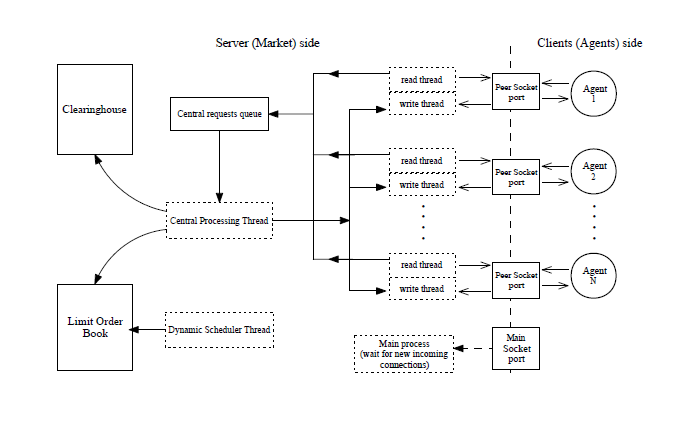
\includegraphics[width=\textwidth]{SERVER}
\caption{Server diagram reproduced from \citet{guo2005}. Solid borders rectangles represents essential data structures residing in computer memory, while dashed represents major processes/threads running on the server. A think arrow link between a thread and a data structure suggests that the thread can access and modify the content of the data structure.}
\label{fig:server}
\end{center}
\end{figure}

Figure \ref{fig:client} identifies the key threads and data structures that are associated with an artificial agent. The two interacting part of agent, the "physical body part" and the "head (or brain) part" provides  scalability in software design. In simulation framework by \citet{guo2005}, experimenting with a new agent, one simply
needs to code the agent's logic into the brain part, plug the brain part into the body and start the simulation.

\begin{figure}[ht]
\begin{center}
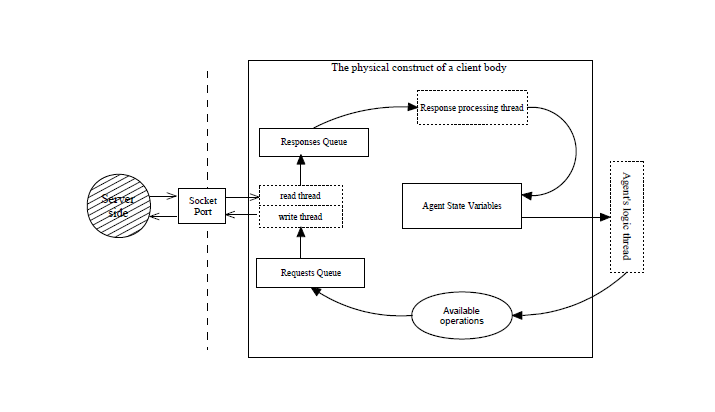
\includegraphics[width=\textwidth]{CLIENT}
\caption{Structure diagram for an artificial client reproduced from \citet{guo2005}. Rectangles with dashed
borders represent threads and those with solid borders represents data structures. An oval represents a set of available operations for the agent to interact with the market.}
\label{fig:client}
\end{center}
\end{figure}

Choice of programming language is the toughest part, when it comes to considering complexity. If the desired simulation system involves complex structure and multiple processes, an object-oriented language (such as C++,
Java and Python) is likely to be the only feasible choice \citep{guo2005}. Java and Python are more desirable than the standard C++ language, when it comes to library support, must essential requirement for complex simulation. In terms of performance, where simulations can be very computationally intensive, C++ can result in a faster and more efficient simulation than Java and Python. \citet{guo2005} ABM architecture is implemented using the Python programming language, provide a distributed computing environment and multithreaded approach with a client/server type of architecture that mimics the exchange/trader setting of real financial markets.

\subsection{Others}
The market is flooded with large number of ABM having different architecture, simulation methodologies and implementation environment. According to \cite{macal2010}, It can be categorized into library-oriented, integrated development environment (IDE) and hybrid. In the library-oriented approach, the agent modelling tool consists of a library of routines organized into an application programming interface (API). Example in the market are, Repast Suite \footnote{RePast (Recursive Porous Agent Simulation Toolkit), \url{http://repast.sourceforge.net/}}, Swarm \footnote{SDG (Swarm Development Group), \url{http://www.swarm.org/.}} and MASON \footnote{MASON (Multi-Agent Simulation of Neighbourhoods), \url{http://cs.gmu.edu/~eclab/projects/mason/}} build on Java archives. The IDE approach uses a code or model editing program to organize model construction. NetLogo\footnote{NetLogo, \url{http://ccl.northwestern.edu/netlogo/index.shtml}}, but suffers from scalability issues as code grows large and larger. The hybrid approach allows modelers to use the environment as either a stand-alone library or a factored multiple-file IDE. Anylogic \footnote{Anylogic, Multimethod Simulation Software, \url{http://www.anylogic.com/}} falls in this category. General programming languages such as Python, Java, and C++, and C also can be used, but development from scratch can be prohibitively expensive. For complete list of software, please refer \citet{Allan2009}. 

\section{Conclusions}\label{sec:con}
Though the research on interaction between HFT and ABM is very shallow, but this paper is an attempt to review some representative Agent-Based Models taking account of High Frequency Trading (HFT) strategies. The studies on building blocks of ABM (agent ecology, trading strategies and marker mechanism) provides us foundation to understand concentrated risk due to interaction of trading strategies employed by various market participants including HFT, which may be applied to understand "flash crash" like event. We tried to provide literature review of the representative model, but there are still lot to be incorporated to make the best model.


\newpage
\bibliographystyle{plainnat} 
\bibliography{ref}

\end{document}

